\documentclass[11pt]{proc}
\usepackage{graphicx}

\begin{document}
\onecolumn

\section{Results}

Starting from $R=0.25, H=0.25, Rm=60, Da=5\times10^-5$, $R$ was varied in steps of $0.006$ ($2.5\% of 0.25$). \\

When R was decreased, the new initial value of $b$ was set to the steady state value of $a$ for $R+0.006$. If at any point I got stuck in a state of $a_{relaxed} = b$ for successive timesteps I would increase $b$ by $1\%$ and continue.

The plot below shows the value of $\psi_{max}$ for a range of $R$. All other parameters were kept the same.

Calculations were performed on a 40x40 grid, and each new steady state took on avergae a couple of minutes to be found.


\begin{figure}[h]
    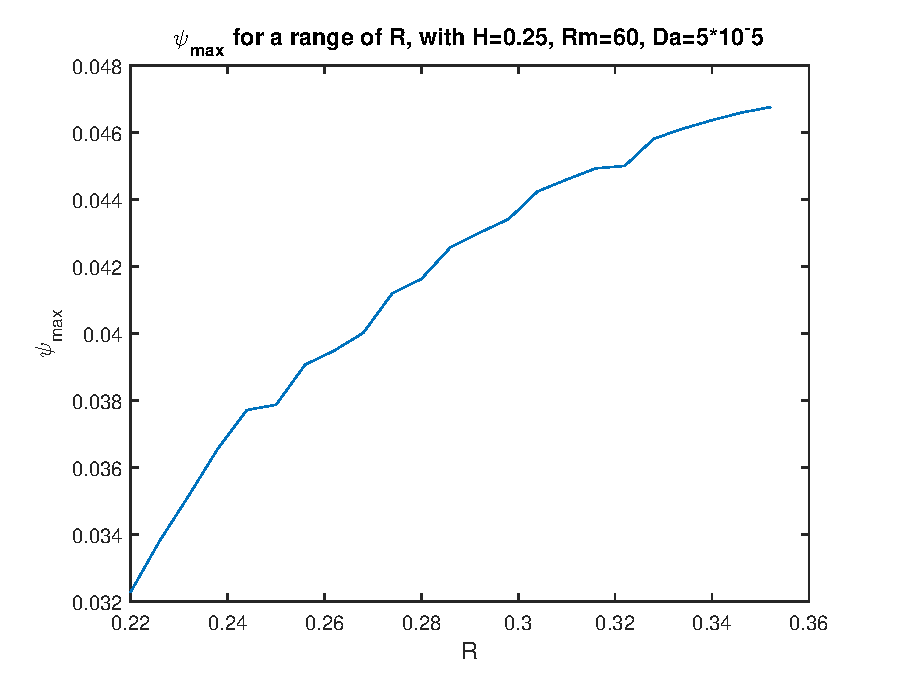
\includegraphics{max_psi_function_of_R}
\end{figure}




\end{document}